\documentclass[addpoints, 11pt]{exam}

\usepackage{amsmath}
\usepackage{amssymb}
\usepackage{graphicx}
\usepackage{fancyhdr}
\usepackage{multicol}
\usepackage{hyperref}

\pagestyle{fancy}% Change page style to fancy
\rhead{{\bf Assigned:} Monday, January 26, 2015 \\{\bf Due:} Wednesday, February 4, 2015}

\newcommand{\ds}{\displaystyle}
\newcommand{\lm}{\lim\limits}
\newtheorem{Definition}{Definition}

\begin{document}
\vspace{100mm}
\begin{center} \Large
MTH 371: Homework 1 \\ Scilab and Programming Introduction\normalsize
\end{center}
\ \\
\noindent GENERAL HOMEWORK GUIDELINES: 
\begin{itemize}
\item On the very first page of your homework, provide your name, date, and homework number.\vspace{-2mm}
\item Homework will be graded in part on neatness, organization, and completeness of solutions. Multiple pages MUST BE STAPLED. \vspace{-2mm}
\item Attach all Scilab code, output, and plots to the page \emph{immediately following} each problem. \vspace{-2mm}
\item Clearly label all plots (title, $x$-axis, $y$-axis, legend). Use the ``subplot" when needed
\end{itemize}


\begin{questions}
%%%%%%%%%%%%%%%%%%%%%%%%%%%%%%%%%%%%%%%%%%%%
% matrix operations practice
%%%%%%%%%%%%%%%%%%%%%%%%%%%%%%%%%%%%%%%%%%%%
\question With matrices and vectors
$$
A = \left(
\begin{array}{rr}
10 & -3 \\
4 & 2
\end{array} \right) , \quad
B = \left(
\begin{array}{rr}
1 & 0 \\
-1 & 2
\end{array} \right) , \quad
\vec{v} = \left(
\begin{array}{r}
1  \\
2
\end{array} \right) , \quad
\vec{w} = \left(
\begin{array}{r}
1  \\
1
\end{array} \right) ,
$$
compute the following \emph{both} by hand and in Scilab. For the Scilab computations, use the ``diary" command to record your session. Here, $T$ denotes the matrix or vector transpose.
\begin{parts}
\begin{multicols}{2}
\part $\ds \vec{v}^T\vec{w}$
\part $\ds \vec{v}\vec{w}^T$
\part $\ds A\vec{v}$
\part $\ds A^T\vec{v}$
\part $\ds AB$
\part $\ds BA$
\part $\ds A^2 ( = AA)$
\part the vector $\vec{y}$ for which $\ds  B\vec{y}=\vec{w}$
\part the vector $\vec{x}$ for which $\ds  A\vec{x}=\vec{v}$
\end{multicols}
\end{parts}

%%%%%%%%%%%%%%%%%%%%%%%%%%%%%%%%%%%%%%%%%%%%
% magic squares, matrix indexing and sums
%%%%%%%%%%%%%%%%%%%%%%%%%%%%%%%%%%%%%%%%%%%%
\question A magic square is a $n\times n$ matrix constructed with integers 1 through $n^2$ (each number used exactly once) with equal row, column, and diagonal sum. 
\begin{parts}
\part What do you expect all of the row, column, and diagonal sums to be for a $n\times n$ magic square? Explain why. 
\part Using the ``diary" command to record your session, complete the following steps in \emph{as few commands as possible}. Make sure to take advantage of matrix indexing and the \verb1sum1 command.
\begin{subparts}
\subpart Create a $4\times 4$ magic square matrix via the command \verb1A=testmatrix('magi',4)1.
\subpart Check all the row sums.
\subpart Check all the column sums.
\subpart Check both the diagonal sums.
\end{subparts}
\part Visualize the $n\times n$ magic squares via the command \verb1surf(A)1 for $n=8,9,10,11$. Use the subplot commands to include these four plots within a single figure.
\end{parts}

%%%%%%%%%%%%%%%%%%%%%%%%%%%%%%%%%%%%%%%%%%%%%
% graphing practice
%%%%%%%%%%%%%%%%%%%%%%%%%%%%%%%%%%%%%%%%%%%%%
\question 
\begin{parts}
\part Write a script file which constructs a vector $x$ consisting of 200 evenly spaced points on the interval $[0,2\pi]$, then plot $y=\sin(kx)$ for $k=1,2,3,4,5$ all on the same plot. Be sure to give your graph a title, label the $x$ and $y$ axis, display a legend, and distinguish each curve. 
\part Using the ``subplot" command, create a single figure including plots $y=\sin(k)$ for $k$ integers ranging from 0 to 1000, and also $y=\sin(k)$ for $k$ integers ranging from 0 to 10000. (For more, see Richert's paper posted on the D2L website).
\end{parts}


%%%%%%%%%%%%%%%%%%%%%%%%%%%%%%%%%%%%%%%%%%%%
% golden ratio basic and graphing
%%%%%%%%%%%%%%%%%%%%%%%%%%%%%%%%%%%%%%%%%%%%
\question The golden ratio $\phi$ shows up in many places in mathematics (and nature!). This ratio gets its name from the golden rectangle shown below. This rectangle has the property that removing a square leaves a smaller rectangle of the same proportions as the original. 
\begin{center}
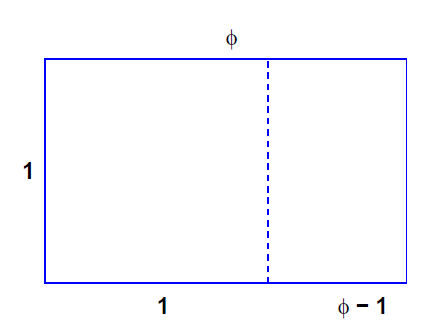
\includegraphics[width=2.25in, height=1.5in]{goldenRect.png} 
\end{center}
Taking the ratio of corresponding sides gives $\ds \frac{1}{\phi}=\frac{\phi-1}{1}$. Rearranging, we have the quadratic equation $\phi^2-\phi-1=0$.
\begin{parts}
\part Find the two roots of this quadratic by hand. The positive root is the golden ratio.
\part Write a Scilab script which plots this quadratic function. Find and plot its zeros via the ``roots" command.
\end{parts}


%%%%%%%%%%%%%%%%%%%%%%%%%%%%%%%%%%%%%%%%%%%%
% golden ratio continued fraction, for loops
% move to lecture?
%%%%%%%%%%%%%%%%%%%%%%%%%%%%%%%%%%%%%%%%%%%%
%\question A continued fraction is an expression of the form
%\[
%a_0 + \frac{1}{a_1+\frac{1}{a_2+\frac{1}{a_3+\cdots}}}.
%\]
%\begin{parts}
%\part If $a_k=1$ for all $k$, the resulting continued fraction is $\phi$, the golden ratio. That is,
%\[
%\phi =1 + \frac{1}{1+\frac{1}{1+\frac{1}{1+\cdots}}}.
%\]
%Use ideas of the previous problem to explain why this is true.
%\part Write a Scilab function \verb1phiApx = goldfrac(n)1 which computes the truncated continued fraction of part (a) including $a_0$ through $a_n$ terms.
%\end{parts}

%%%%%%%%%%%%%%%%%%%%%%%%%%%%%%%%%%%%%%%%%%%%
% fibonacci, for loop, indexing, array division
%%%%%%%%%%%%%%%%%%%%%%%%%%%%%%%%%%%%%%%%%%%%
\question The Fibonacci Sequence is defined recursively as
\[
f_n = f_{n-1} + f_{n-2}, \quad f_1=1, f_2=2.
\]
\begin{parts}
\part Write a Scilab function \verb1f = fibonacci(n)1 returns array \verb1f1 of the first $n$ Fibonacci numbers. (Hint: Use a for loop.)
\part Write a Scilab script which computes the term-by-term growth rate of the Fibonacci sequence. To do this, compute the first 40 Fibonacci numbers via the function in part (a), then compute ratios $\ds \phi_n=\frac{f_{n+1}}{f_n}$. You can compute all these ratios in a single line of code. What does $\phi_n$ seem to approach?
\part Record the following session in Scilab via the ''diary" command. 
\begin{subparts}
\subpart Enter the statements
\[
A = [1~ 1; 1~ 0];~ X = [1~ 0; 0~ 1];
\]
then the statement
\[
X=A*X
\]
Now, repeatedly press the up arrow key, followed by the enter key. What happens? Explain why.
\subpart Use Scilab to compute the eigenvalues of matrix $A$. What is the result and why?
\end{subparts}
\end{parts}
\pagebreak

%%%%%%%%%%%%%%%%%%%%%%%%%%%%%%%%%%%%%%%%%%%%
% 3n+1 sequence, while loop and if statements
%%%%%%%%%%%%%%%%%%%%%%%%%%%%%%%%%%%%%%%%%%%%
\question A famous unsolved problem in number theory the $3n+1$ problem and is as follows. Start with positive integer $n$. Repeat the following steps.
\begin{itemize}
\item If $n=1$, stop.
\item If $n$ is even, replace it with $\frac{n}{2}$.
\item If $n$ is odd, replace it with $3n+1$.
\end{itemize}
For example, starting with $n=7$ produces
\[
7, 22, 11, 34, 17, 52, 26, 13, 40, 20, 10, 5, 16, 8, 4, 2, 1.
\]
The sequence terminates after 17 steps. The unanswered question is, does this process always terminate?
\begin{parts}
\part Write a Scilab function \verb1y = threenplus11\verb1(n)1 returning array \verb1y1 which is the entire sequence generated by positive integer \verb1n1. (Hint: Use a while loop and if statements.)
\part Write a Scilab script which computes the sequences generated by integers 2 through 10, and display them all on the same plot.
\part The $3n+1$ sequence has a particular shape for $n$ starting at $5,10,20,40,80,\dots$ Why is this?
\part The graphs of $3n+1$ sequences are all quite similar for $n=108, 109, 110$. Why?
\end{parts}

%%%%%%%%%%%%%%%%%%%%%%%%%%%%%%%%%%%%%%%%%%%%
% prime spirals
%%%%%%%%%%%%%%%%%%%%%%%%%%%%%%%%%%%%%%%%%%%%
\question OPTIONAL challenge problem. Consider organizing the positive integers in an $n\times n$ array in a spiral fashion as illustrated in the below picture. Note the prime numbers are highlighted in red. The location of these primes forms what is called an Ulam prime spiral. By plotting points, this spiral is hilighted in the next image for the $200 \times 200$ case. Write a Scilab script which replicates the second image. Generate your own image for the  $400 \times 400$ and  $800 \times 800$ cases. For more on Ulam prime spirals, see \url{http://blogs.mathworks.com/cleve/2015/01/05/prime-spiral/}.
\begin{center}
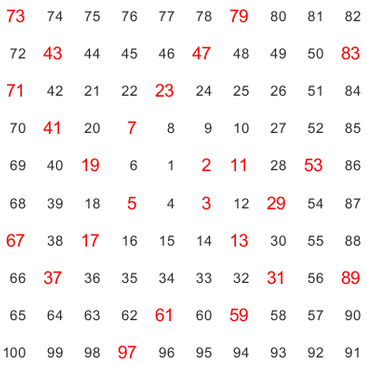
\includegraphics[width=2.5in, height=2.5in]{prime.png} \quad
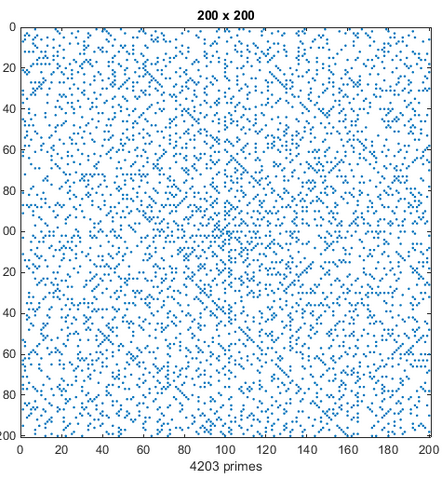
\includegraphics[width=2.5in, height=2.5in]{spiral.png}
\end{center}

\end{questions}
\end{document} 